\documentclass[12pt, a4paper]{article}
\usepackage[a4paper, mag=1000, left=1.5cm, right=1.5cm, top=2cm, bottom=2cm, headsep=0.7cm, footskip=1cm]{geometry}
\usepackage{iftex}
\ifXeTeX
  % XeLaTeX / Tectonic: Computer Modern Unicode (тот же вид, что и T2A в pdfLaTeX)
  \usepackage{fontspec}
  \setmainfont{cmunrm.otf}[BoldFont=cmunbx.otf, ItalicFont=cmunti.otf, BoldItalicFont=cmunbi.otf]
  \setsansfont{cmunss.otf}[BoldFont=cmunsx.otf, ItalicFont=cmunsi.otf, BoldItalicFont=cmunso.otf]
  \setmonofont{cmuntt.otf}[BoldFont=cmuntb.otf, ItalicFont=cmunit.otf, BoldItalicFont=cmuntx.otf]
\else
  \usepackage[T2A]{fontenc}
  \usepackage[utf8]{inputenc}
\fi
\usepackage[english,russian]{babel}
\usepackage[hidelinks]{hyperref}
\usepackage{graphicx}
\usepackage{amsmath}
\usepackage{float}
\usepackage{titlesec}
\usepackage{caption}
\usepackage{fvextra}
\usepackage{array}
\newcolumntype{L}[1]{>{\raggedright\arraybackslash}p{#1}}
\DefineVerbatimEnvironment{code}{Verbatim}{fontsize=\small,breaklines=true,breakanywhere=true,breaksymbolleft={}}

\captionsetup{labelsep=period}

\titleformat{\section}{\Large\bfseries\centering}{}{0em}{}
\renewcommand{\thesection}{}

\begin{document}
\thispagestyle{empty}

\begin{center}
    {\Large\textbf{ФЕДЕРАЛЬНОЕ ГОСУДАРСТВЕННОЕ АВТОНОМНОЕ ОБРАЗОВАТЕЛЬНОЕ УЧРЕЖДЕНИЕ ВЫСШЕГО ОБРАЗОВАНИЯ}}\\
    {\Large\textbf{«НАЦИОНАЛЬНЫЙ ИССЛЕДОВАТЕЛЬСКИЙ УНИВЕРСИТЕТ ИТМО»}}\\[5mm]
    {\large\text{ФАКУЛЬТЕТ ТЕХНОЛОГИЙ ИСКУССТВЕННОГО ИНТЕЛЛЕКТА}}\\[5mm]
    
\includegraphics[scale=0.14]{logo.png}\\[20mm]
    \rule{\textwidth}{0.4mm}\\[3mm]
    {\Large\text{Лабораторная работа №3}}\\[3mm]
    {\Large\text{по дисциплине «Инженерия данных»}}\\[3mm]
    \rule{\textwidth}{0.4mm}
\end{center}

\vfill

\begin{flushright}
    \large Выполнил: \\[2mm]
    Студент группы J3311 \\
    Поладов Селим Бегенджович \\
    ИСУ: 467128
\end{flushright}

\vfill

\begin{center}
    \large Санкт-Петербург \\
    \large 2026
\end{center}

\newpage

\titleformat{\section}{\Large\bfseries\raggedright}{}{0em}{}
\titleformat{\subsection}{\large\bfseries\raggedright}{}{0em}{}
\titlespacing*{\section}{0pt}{10pt}{6pt}
\titlespacing*{\subsection}{0pt}{8pt}{3pt}

\sloppy
\section{1. Развертывание RustFS}

Цель работы в том, чтобы посчитать навыки, пары и тройки навыков своего
варианта двумя независимыми способами по данным из объектного хранилища,
сверить результаты, сравнить подходы по времени и памяти и найти навыки,
которые связаны с зарплатой и различаются по регионам. Вариант 9,
программист, разработчик на мобильных платформах.

Работа выполнена 21 октября 2026 года на macOS, процессор с 12 ядрами,
24 ГБ памяти, Docker Desktop. RustFS 1.0.0 поднят по профилю home из стенда
второго домашнего задания. Один процесс работает с четырьмя папками-дисками
vol1, vol2, vol3 и vol4, схема кодирования EC 2+2. Папки лежат в локальном
каталоге data, ключи доступа в файле .env, который не попадает в отчет и
репозиторий. S3 API доступен на порту 9010, консоль на порту 9011.

\begin{code}
services:
  rustfs-home:
    image: rustfs/rustfs:1.0.0
    container_name: hh-lake-rustfs
    profiles: ["home"]
    env_file: .env
    environment:
      RUSTFS_VOLUMES: /data/vol{1...4}
      RUSTFS_UNSAFE_BYPASS_DISK_CHECK: "true"
      RUSTFS_STORAGE_CLASS_STANDARD: "EC:2"
    ports: ["127.0.0.1:9010:9000", "127.0.0.1:9011:9001"]
    volumes: ["./data:/data"]
\end{code}

\begin{figure}[H]
\centering
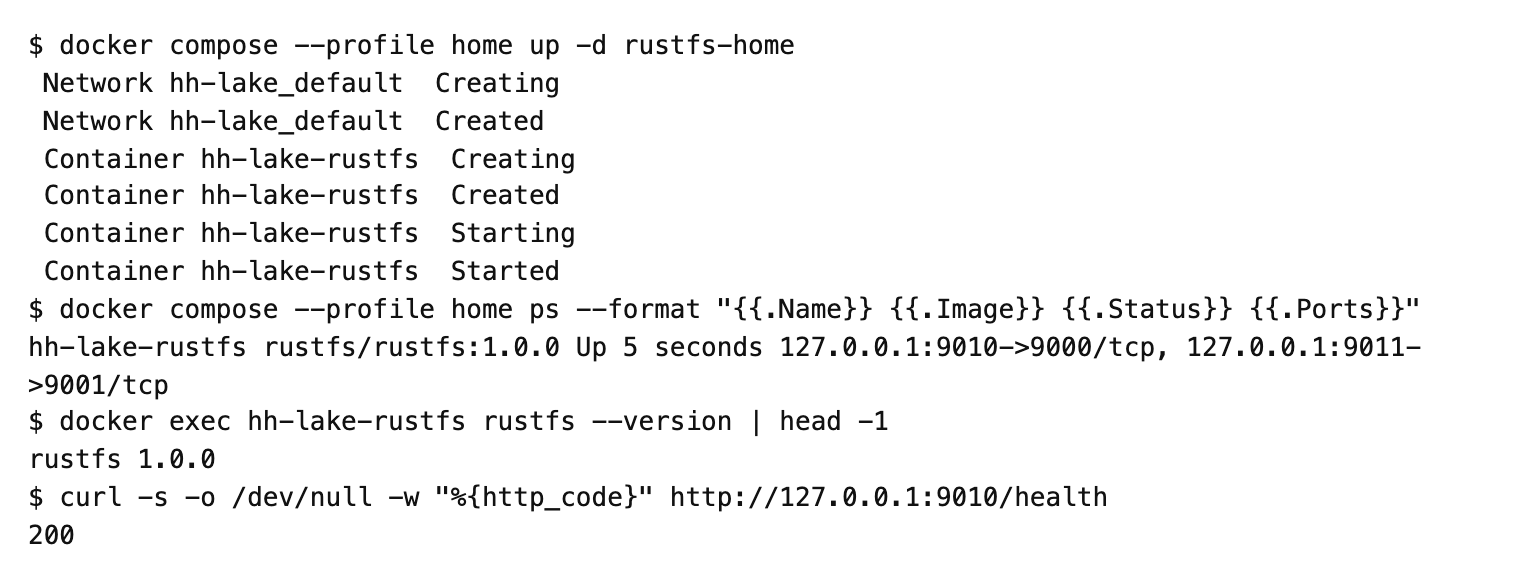
\includegraphics[width=\textwidth]{../screenshots/01_deploy.png}
\caption{Запуск контейнера и проверка RustFS}
\end{figure}

\begin{figure}[H]
\centering
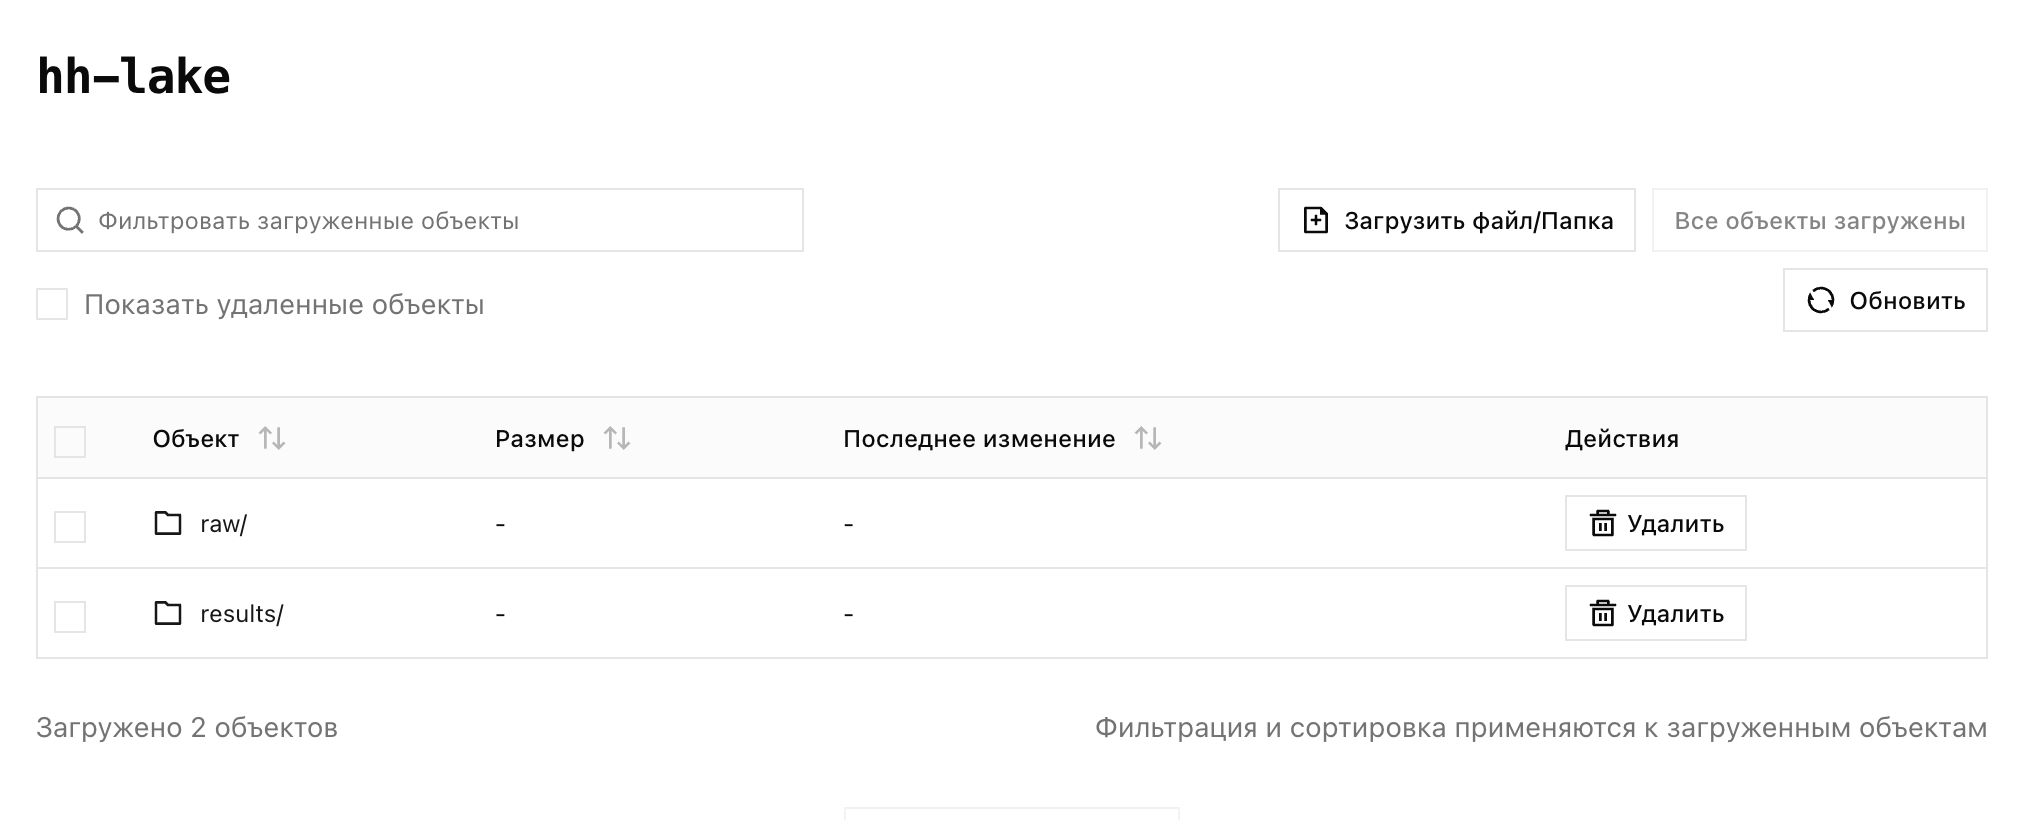
\includegraphics[width=0.85\textwidth]{../screenshots/console_hh_lake.png}
\caption{Бакет hh-lake в консоли RustFS}
\end{figure}

\section{2. Загрузка данных}

Используется предоставленный файл it\_vacancies\_2024.csv с IT-вакансиями
hh.ru за 2024 год. В нем 229388 вакансий, 23 столбца и 847619384 байта.
Каждая запись занимает ровно одну строку файла, всего 229389 строк вместе с
заголовком. Поэтому файл можно делить на части по байтам и выравнивать части
по переводу строки.

Скрипт upload.py загрузил файл в бакет hh-lake как объект
raw/it\_vacancies\_2024.csv через boto3. После загрузки объект прочитан
обратно, SHA256 совпала с локальным файлом.

В бакет загружен полный датасет. Вакансии варианта отбираются при обработке
одним и тем же условием, которое отдельно написано на Python для MapReduce и
на SQL для DuckDB. Так условие варианта проверяется в двух независимых
реализациях.

\begin{figure}[H]
\centering
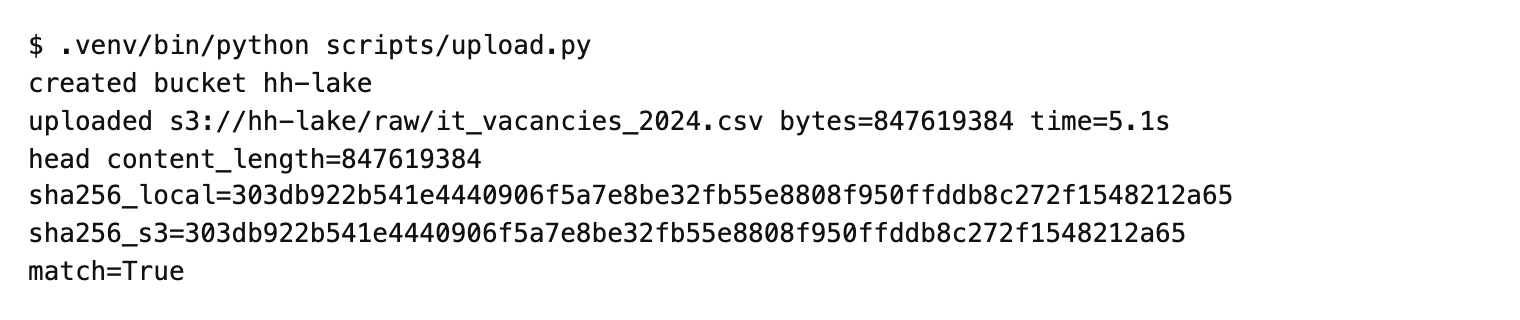
\includegraphics[width=\textwidth]{../screenshots/02_upload.png}
\caption{Загрузка датасета и проверка контрольной суммы}
\end{figure}

\begin{figure}[H]
\centering
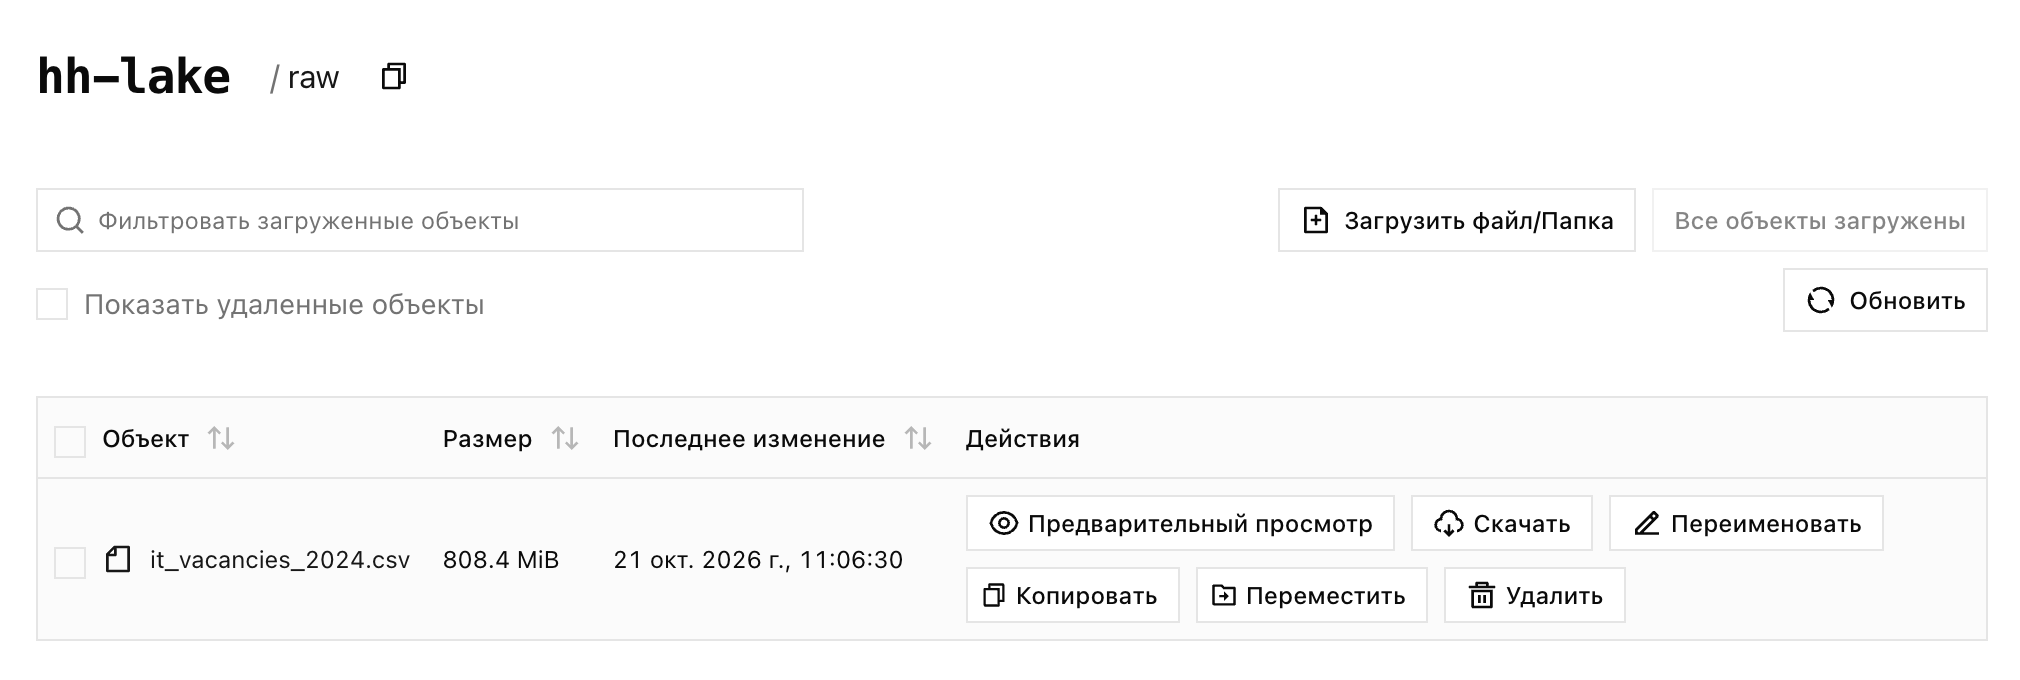
\includegraphics[width=0.85\textwidth]{../screenshots/console_raw.png}
\caption{Объект с датасетом в бакете hh-lake}
\end{figure}

\section{3. Подсчет навыков, пар и троек}

\subsection{Условие варианта и навыки}

Вакансия относится к варианту, если ее роль hh равна
\texttt{Программист, разработчик}, а в названии есть мобильная платформа.
Название приводится к нижнему регистру. С начала слова ищутся android,
андроид, мобильн, flutter, флаттер, xamarin, swift, react native,
objective-c и kotlin multiplatform. Отдельными словами ищутся ios, айос,
mobile, ionic и kmp. Граница слова задана явно классом символов, поэтому
одно и то же регулярное выражение одинаково работает в Python и в DuckDB.
Kotlin без мобильной платформы в условие не входит, потому что на Kotlin
пишут и серверные приложения, например в вакансиях Java/Kotlin Developer. Условию
соответствует 3771 вакансия, у 2794 из них заполнены ключевые навыки.

\begin{code}
role = 'Программист, разработчик' AND regexp_matches(lower(name),
'(^|[^a-zа-яё0-9])(android|андроид|мобильн|flutter|флаттер|xamarin|swift|react.native|objective.c|kotlin multiplatform)|(^|[^a-zа-яё0-9])(ios|айос|mobile|ionic|kmp)([^a-zа-яё0-9]|$)')
\end{code}

Навыки берутся из столбца key\_skills. Строка делится по точке с запятой,
пробелы по краям убираются, навык приводится к нижнему регистру, повторы
внутри вакансии удаляются, навыки сортируются. Нижний регистр нужен, потому
что один навык записан по-разному, например Kotlin, kotlin и KOTLIN. Пары и
тройки это сочетания разных навыков одной вакансии в порядке сортировки.
Частота сочетания равна числу вакансий, в которых оно есть.

\subsection{Собственный MapReduce}

Программа mapreduce.py повторяет схему map, shuffle и reduce. Объект
делится по байтам на 26 сплитов по 32 МиБ. Каждая map-задача скачивает свой
сплит из RustFS запросом GET с заголовком Range и читает ответ кусками по
1 МиБ. Строка принадлежит тому сплиту, в котором она начинается, как в
LineRecordReader в Hadoop. Задача пропускает хвост строки предыдущего сплита
и дочитывает свою последнюю строку за границей сплита. Скрипт test\_splits.py
проверил это на локальной копии файла для сплитов 1000003, 7340043 и
33554432 байта. Каждая из 229389 строк обработана ровно один раз.

Функция map разбирает строку CSV, проверяет условие варианта и для каждой
вакансии выдает ключи всех сочетаний из одного, двух и трех навыков со
значением 1. Комбайнер суммирует значения одинаковых ключей внутри map-задачи.
Это допустимо, потому что сумма ассоциативна и коммутативна. Ключ попадает в
одну из четырех партиций по crc32, партиция сортируется и пишется на
локальный диск. Reduce-задача сливает отсортированные партиции всех
map-задач и суммирует значения одного ключа. Задачи работают отдельными
процессами, одновременно не больше восьми. Выход задачи фиксируется
переименованием каталога только после успешной попытки, упавшая попытка
перезапускается до четырех раз.

Предфильтр пропускает разбор CSV для строк, в байтах которых нет текста роли
варианта. Такая строка точно не проходит условие, поэтому результат не
меняется. Текст роли есть в 87803 строках из 229389, остальные строки
не разбираются.

\begin{code}
for pos, line in lines:                          # строки своего сплита
    if line is None or ROLE_BYTES not in line:   # предфильтр
        continue
    row = next(csv.reader([line.decode('utf-8')]))
    if not in_variant(row):
        continue
    sk = skills_of(row)                          # нормализованные навыки
    for k in (1, 2, 3):
        for combo in combinations(sk, k):
            key = (k,) + combo
            parts[part_of(key, reducers)][key] += 1   # комбайнер
\end{code}

\begin{figure}[H]
\centering
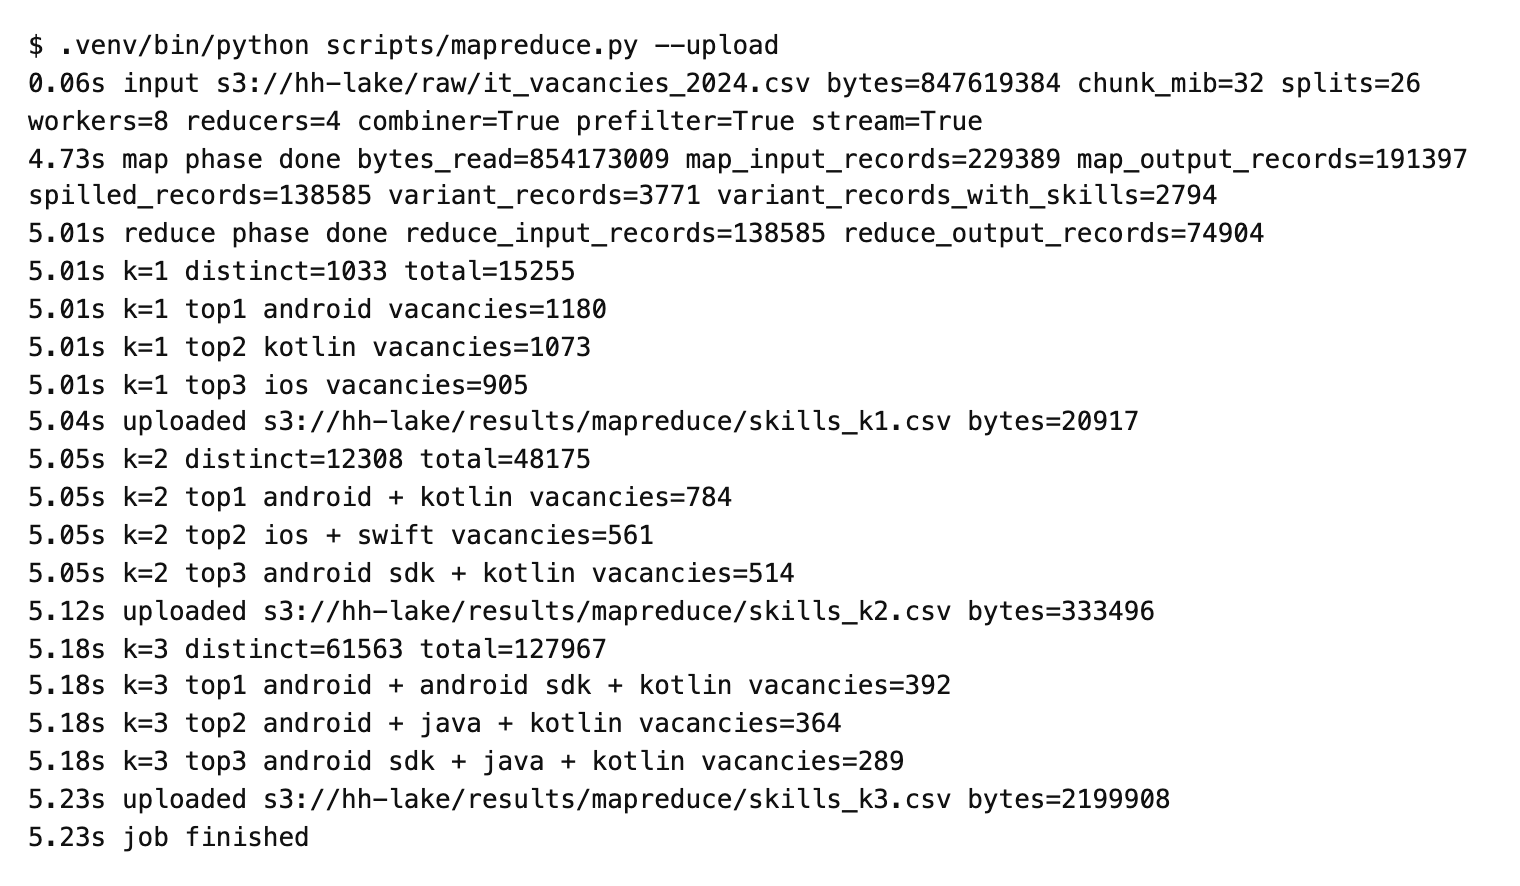
\includegraphics[width=\textwidth]{../screenshots/03_mapreduce.png}
\caption{Запуск MapReduce с записью результатов в hh-lake}
\end{figure}

Счетчики задачи согласованы между собой. На вход map пришли 229389 строк
вместе с заголовком, условию соответствуют 3771 вакансия. Map выдал 191397
пар ключ и значение, это сумма 15255, 48175 и 127967 по трем размерам
сочетаний. Комбайнер сократил данные шаффла до 138585 записей. Reduce выдал
74904 ключа, это 1033 навыка, 12308 пар и 61563 тройки.

\subsection{SQL в DuckDB}

Скрипт duckdb\_skills.py читает тот же объект s3://hh-lake/raw/it\_vacancies\_2024.csv
через расширение httpfs. Условие варианта и нормализация навыков записаны в
SQL. Пары и тройки получаются соединением таблицы навыков с самой собой по
вакансии с условием \texttt{a.skill < b.skill}.

\begin{code}
CREATE TABLE seg AS
SELECT vacancy_id, area, name, experience, schedule,
       salary_from, salary_to, currency, gross,
       list_sort(list_distinct(list_filter(
           list_transform(string_split(key_skills, ';'), x -> lower(trim(x))),
           x -> x <> ''))) AS skills
FROM read_csv('s3://hh-lake/raw/it_vacancies_2024.csv',
              header = true, all_varchar = true)
WHERE role = 'Программист, разработчик'
  AND regexp_matches(lower(name), '<шаблон варианта>');
CREATE TABLE ex AS SELECT vacancy_id, unnest(skills) AS skill FROM seg;
SELECT a.skill AS skill_1, b.skill AS skill_2, c.skill AS skill_3,
       count(*) AS vacancies
FROM ex a JOIN ex b ON a.vacancy_id = b.vacancy_id AND a.skill < b.skill
          JOIN ex c ON b.vacancy_id = c.vacancy_id AND b.skill < c.skill
GROUP BY ALL ORDER BY vacancies DESC, skill_1, skill_2, skill_3;
\end{code}

\begin{figure}[H]
\centering
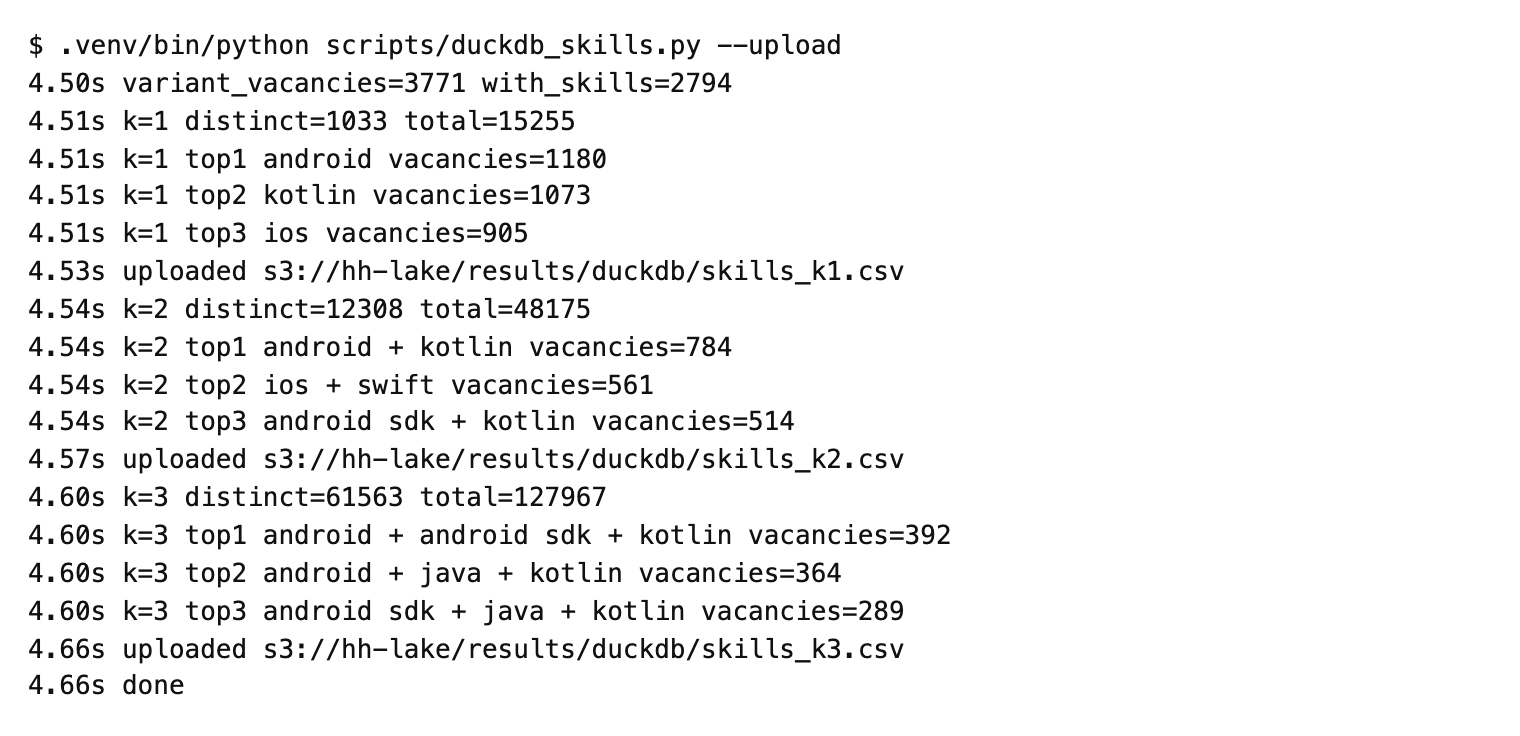
\includegraphics[width=\textwidth]{../screenshots/04_duckdb.png}
\caption{Тот же расчет в DuckDB}
\end{figure}

\subsection{Результаты и рост числа сочетаний}

Самые частые навыки варианта android в 1180 вакансиях, kotlin в 1073, ios в
905, git в 834 и swift в 717. Самые частые пары android + kotlin в 784
вакансиях, ios + swift в 561 и android sdk + kotlin в 514. Самые частые
тройки android + android sdk + kotlin в 392 вакансиях, android + java +
kotlin в 364 и android sdk + java + kotlin в 289. Рынок делится на два
нативных стека, Android на Kotlin и Java и iOS на Swift, и меньший сегмент
кроссплатформенной разработки на Flutter и React Native.

Различных сочетаний становится намного больше с ростом размера. Навыков
1033, пар 12308, троек 61563. Сумма частот растет так же, 15255, 48175 и
127967. Причина в числе сочетаний внутри одной вакансии. Вакансия с $n$
навыками дает $n(n-1)/2$ пар и $n(n-1)(n-2)/6$ троек. При медиане 5 навыков
это 10 пар и 10 троек, а вакансия с 28 навыками дает 378 пар и 3276 троек.
Поэтому 9,6 процента вакансий, где навыков не меньше 10, дают 68,3 процента
всех троек. Суммы $C(n,k)$ по вакансиям точно совпадают с итогами MapReduce.
Большинство длинных сочетаний редкие, один раз встречаются 46 процентов
навыков, 55 процентов пар и 61 процент троек, поэтому число различных ключей
растет быстрее, чем сумма частот.

\begin{figure}[H]
\centering
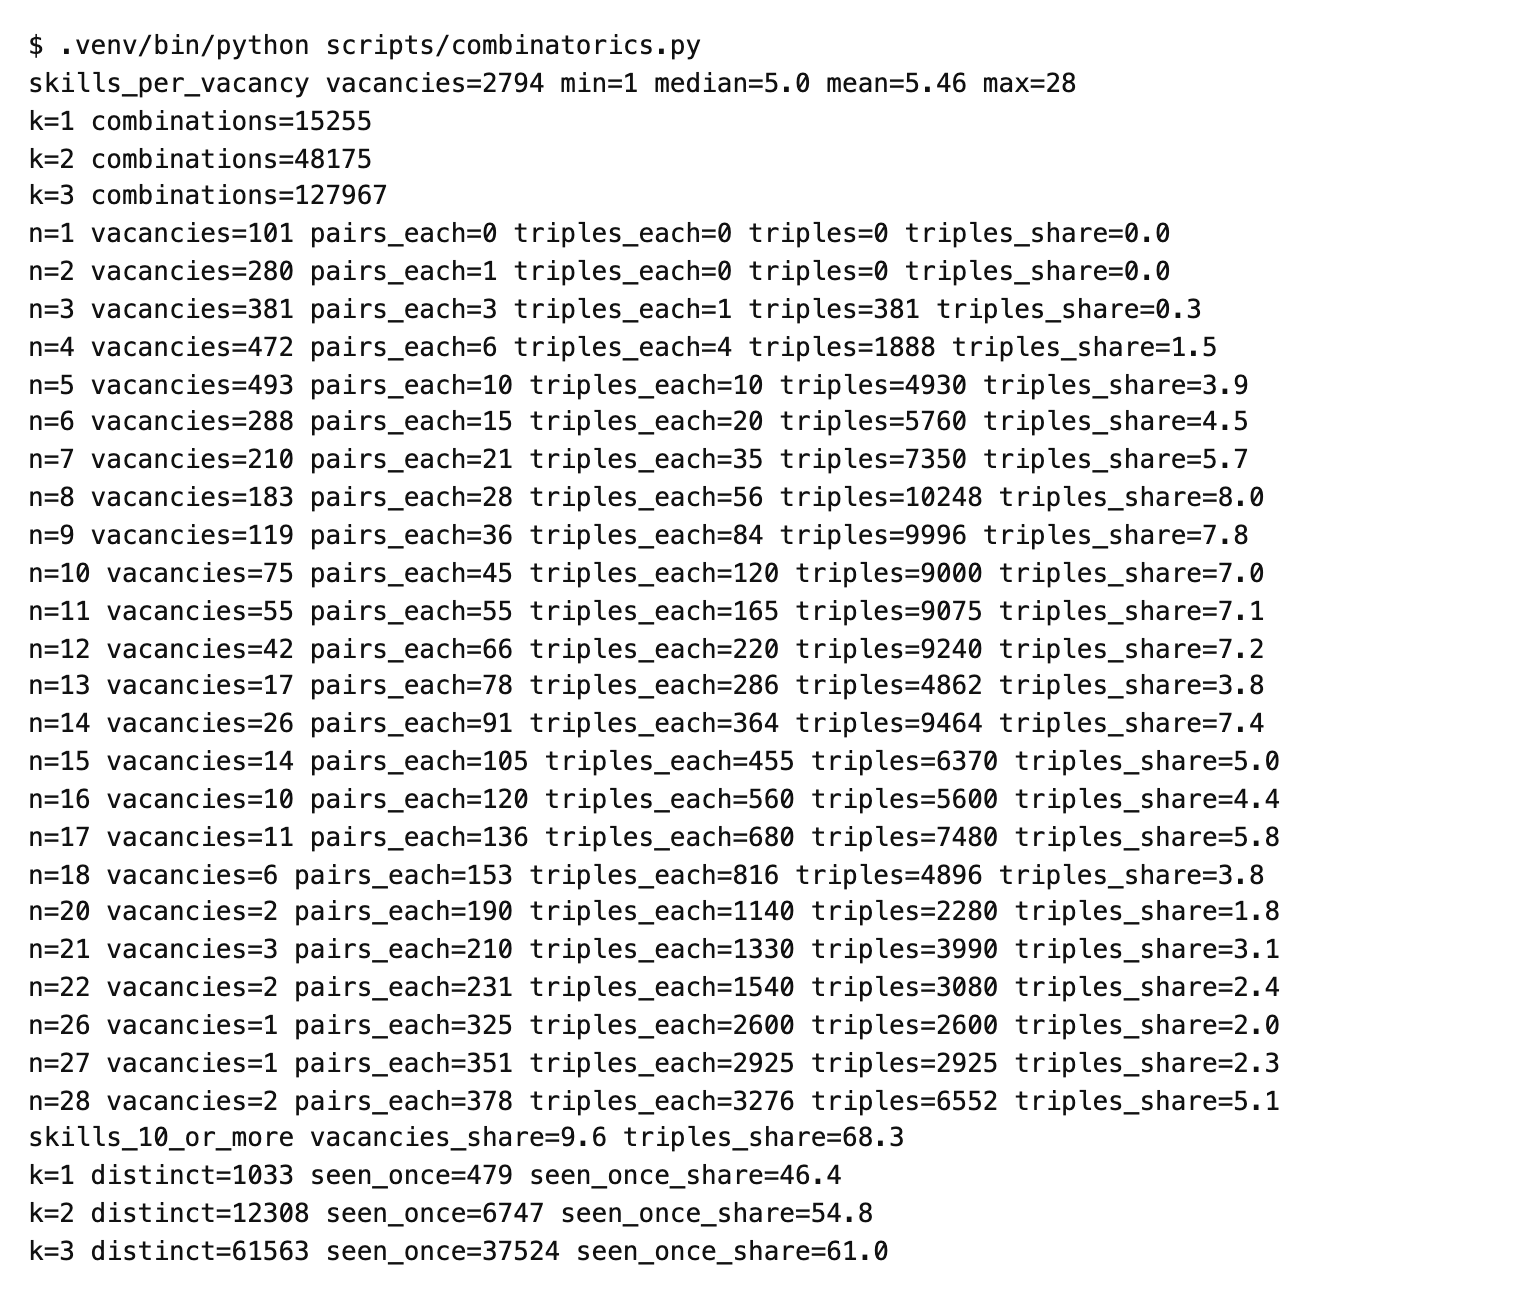
\includegraphics[width=0.9\textwidth]{../screenshots/09_combinatorics.png}
\caption{Число сочетаний в зависимости от числа навыков вакансии}
\end{figure}

Результаты для всех трех размеров сочетаний обоими способами лежат в бакете
hh-lake в папках results/mapreduce и results/duckdb.

\begin{figure}[H]
\centering
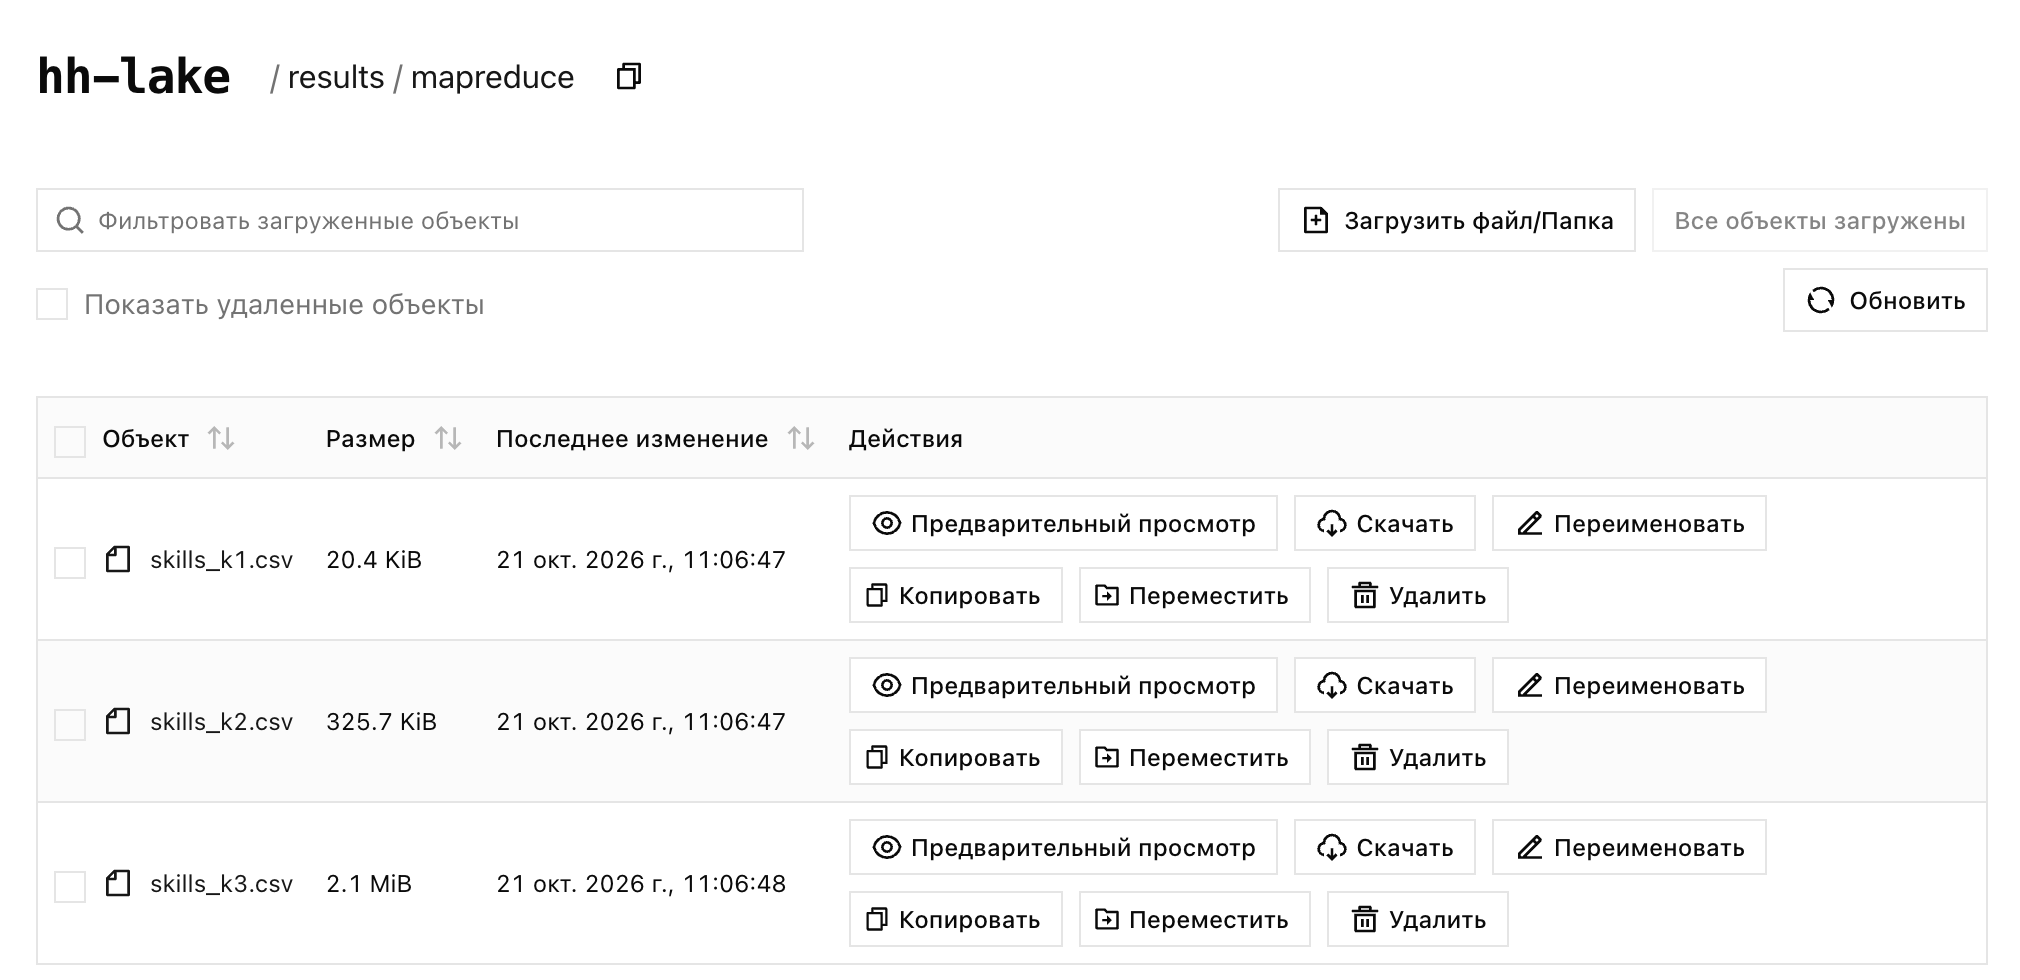
\includegraphics[width=0.85\textwidth]{../screenshots/console_results_mapreduce.png}
\caption{Результаты MapReduce в бакете hh-lake}
\end{figure}

\begin{figure}[H]
\centering
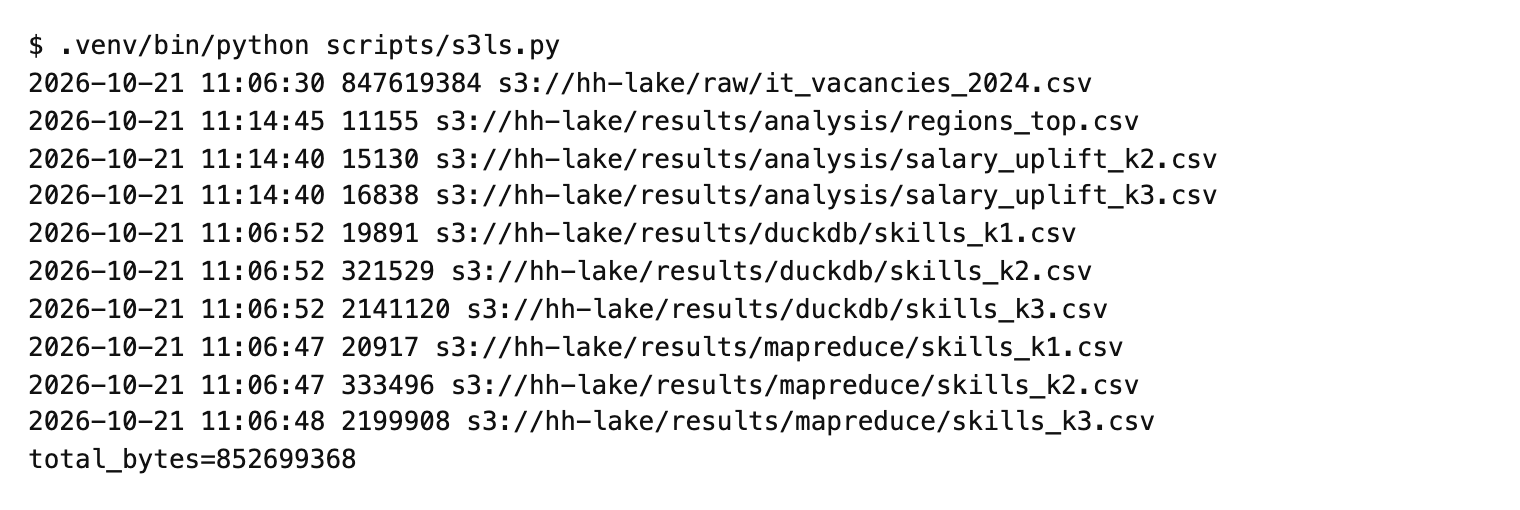
\includegraphics[width=\textwidth]{../screenshots/12_s3ls_final.png}
\caption{Все объекты бакета hh-lake после выполнения работы}
\end{figure}

\section{4. Верификация результатов}

Скрипт verify.py скачивает из hh-lake результаты обоих способов и сравнивает
все строки, то есть сочетания и их частоты. Совпали все 1033 строки навыков,
12308 строк пар и 61563 строки троек, суммы и контрольные хеши. Сами файлы
отличаются по байтам только форматом CSV. У Python окончания строк CRLF, а
DuckDB берет в кавычки значения с решеткой, например c\#. Поэтому
сравниваются разобранные значения, а не байты файлов.

\begin{figure}[H]
\centering
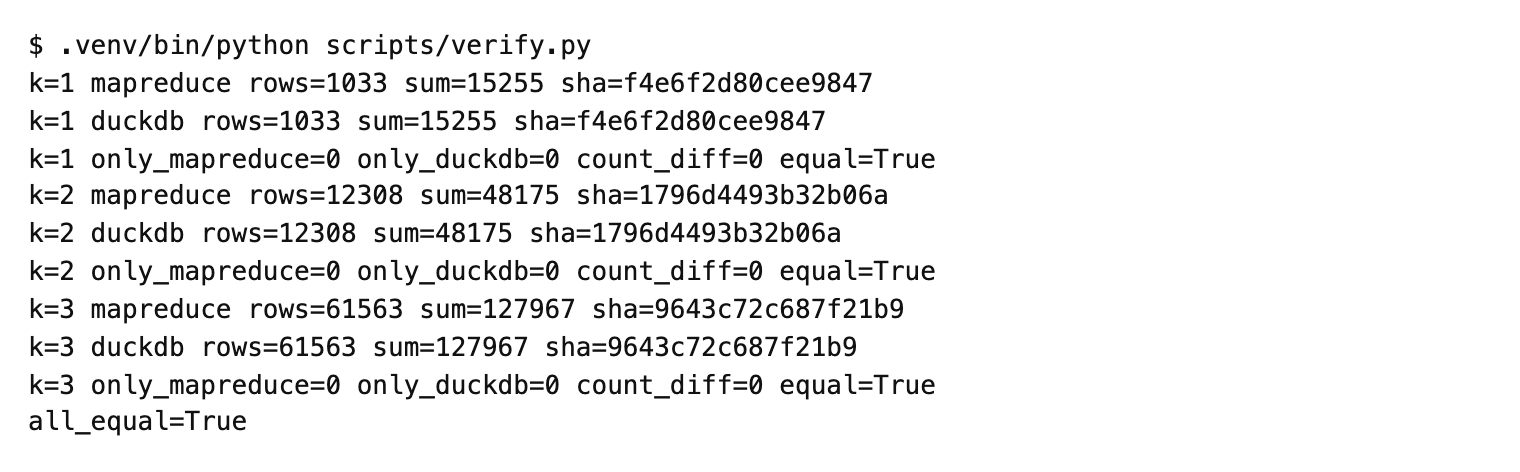
\includegraphics[width=\textwidth]{../screenshots/05_verify.png}
\caption{Полное совпадение результатов MapReduce и DuckDB}
\end{figure}

Отдельно проверен отказ маппера. При запуске с ключом \texttt{--fail-map 5}
процесс map-задачи 5 на первой попытке завершается посреди сплита с кодом 17
и оставляет недописанный выход в каталоге попытки. Планировщик запускает
задачу повторно, вторая попытка проходит. Недописанный выход не
используется, потому что зафиксирован только каталог успешной попытки.
Результаты побайтно совпали с обычным запуском.

\begin{figure}[H]
\centering
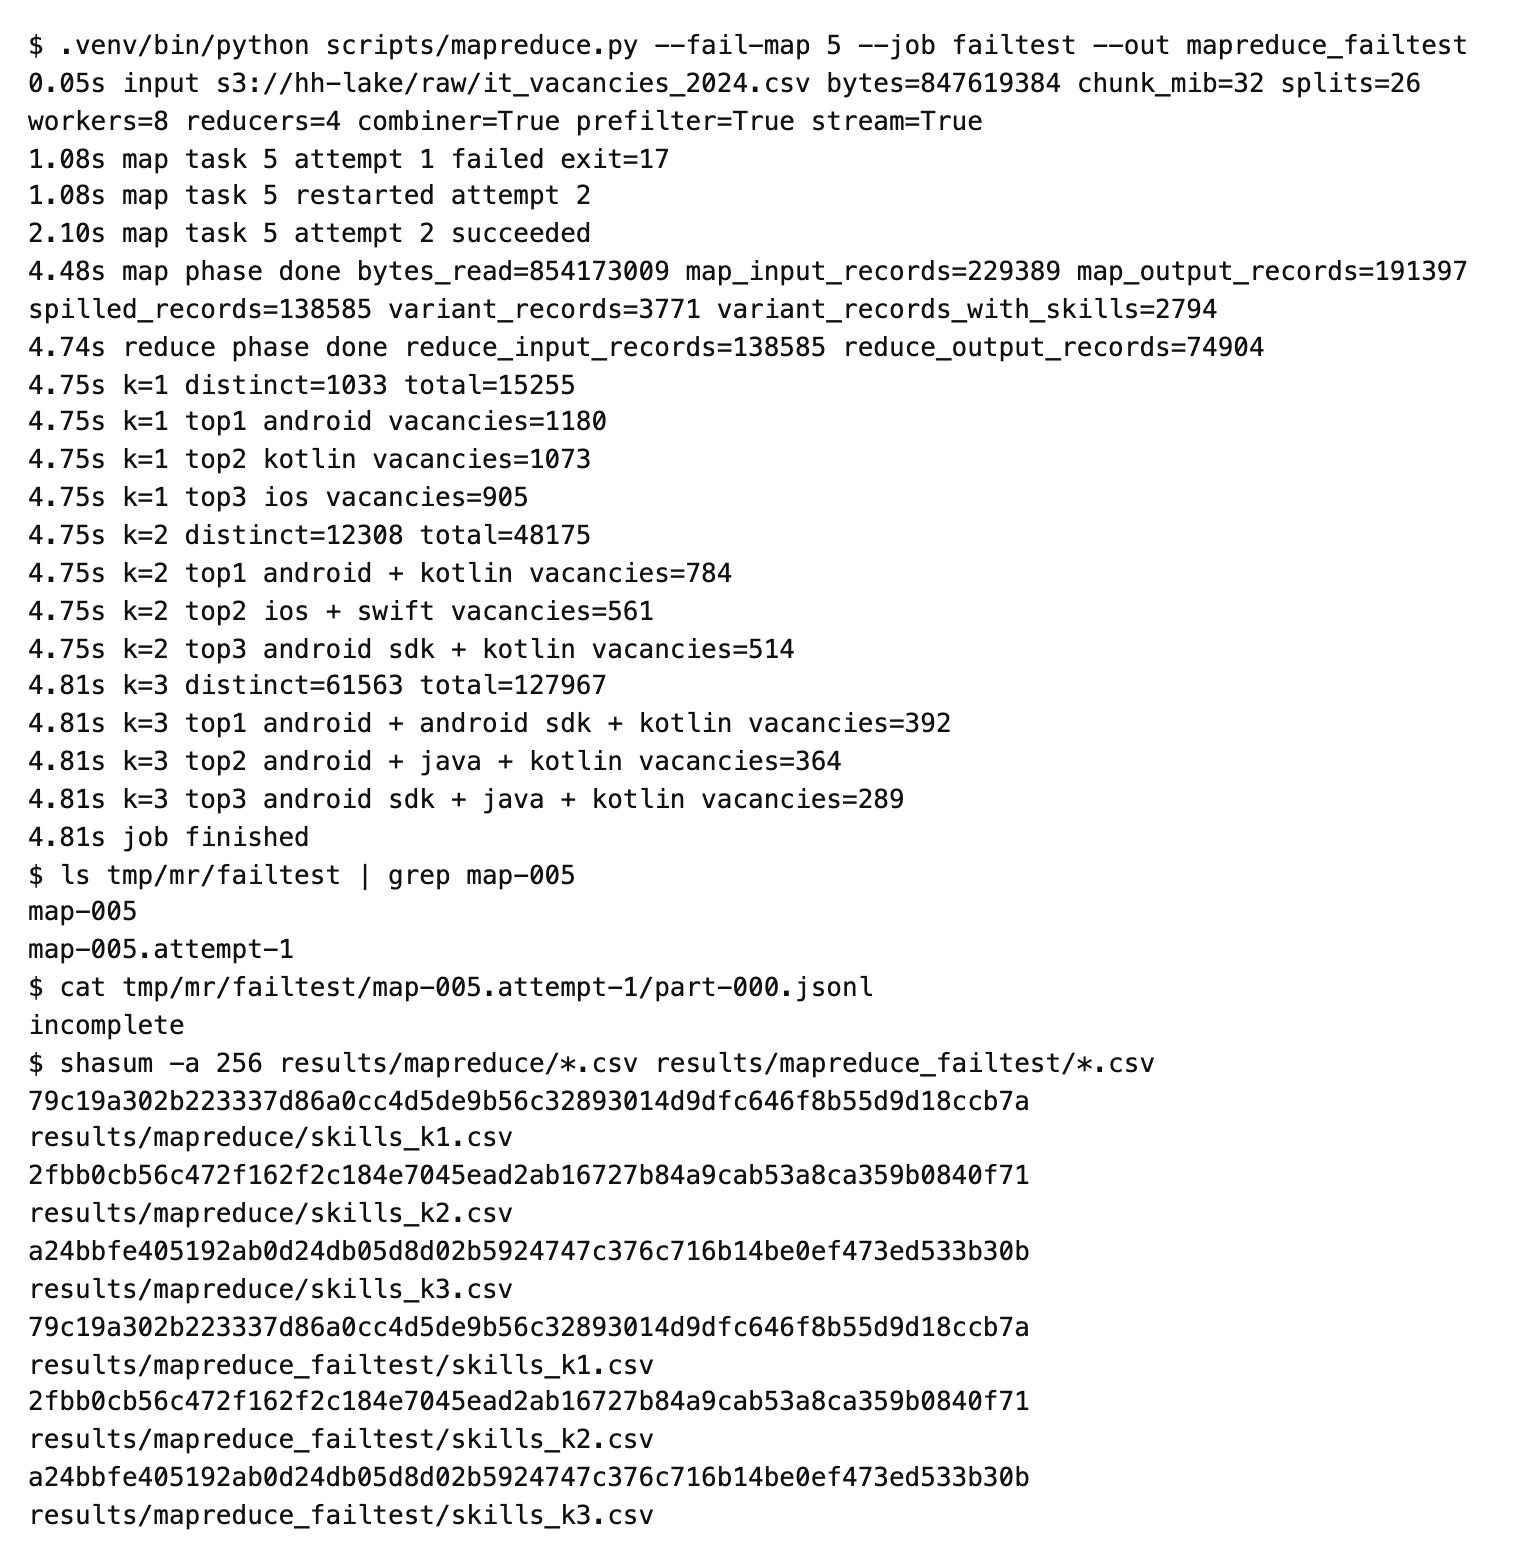
\includegraphics[width=\textwidth]{../screenshots/06_map_failure.png}
\caption{Отказ map-задачи и ее повторный запуск}
\end{figure}

\section{5. Профилирование и оптимизация}

Скрипт profile.py запускает команду пять раз. Время измеряется от запуска до
завершения процесса. Память измеряется каждые 20 мс как сумма RSS процесса и
всех его потомков, берется максимум за запуск. Для MapReduce это важно,
потому что map- и reduce-задачи работают отдельными процессами. Все запуски
читают данные из RustFS.

\begin{table}[H]
\centering
\small
\begin{tabular}{|L{8.3cm}|L{4.0cm}|L{4.0cm}|}
\hline
Конфигурация & Время, с, медиана и разброс & Пик памяти, МиБ, медиана и разброс \\
\hline
MapReduce до оптимизации, 1 процесс, сплит целиком в памяти, без комбайнера и предфильтра & 14,58 (14,46 и 15,47) & 278,0 (259,3 и 280,2) \\
\hline
MapReduce, 1 процесс, потоковое чтение, комбайнер, предфильтр & 11,74 (11,36 и 12,31) & 163,2 (160,9 и 164,1) \\
\hline
MapReduce, 8 процессов, без остальных оптимизаций & 5,85 (5,77 и 6,53) & 1388,2 (1324,1 и 1575,0) \\
\hline
MapReduce после оптимизации, 8 процессов, потоковое чтение, комбайнер, предфильтр & 5,70 (5,28 и 6,06) & 718,4 (669,8 и 735,3) \\
\hline
DuckDB, SQL по тому же объекту & 4,61 (4,49 и 4,82) & 440,3 (417,0 и 477,1) \\
\hline
Только чтение объекта из RustFS в 8 потоков без обработки & 3,78 (3,67 и 3,81) & 113,6 (111,9 и 117,9) \\
\hline
\end{tabular}
\caption{Время и пик памяти, по пять запусков на конфигурацию, в скобках наименьшее и наибольшее значение}
\end{table}

\begin{figure}[H]
\centering
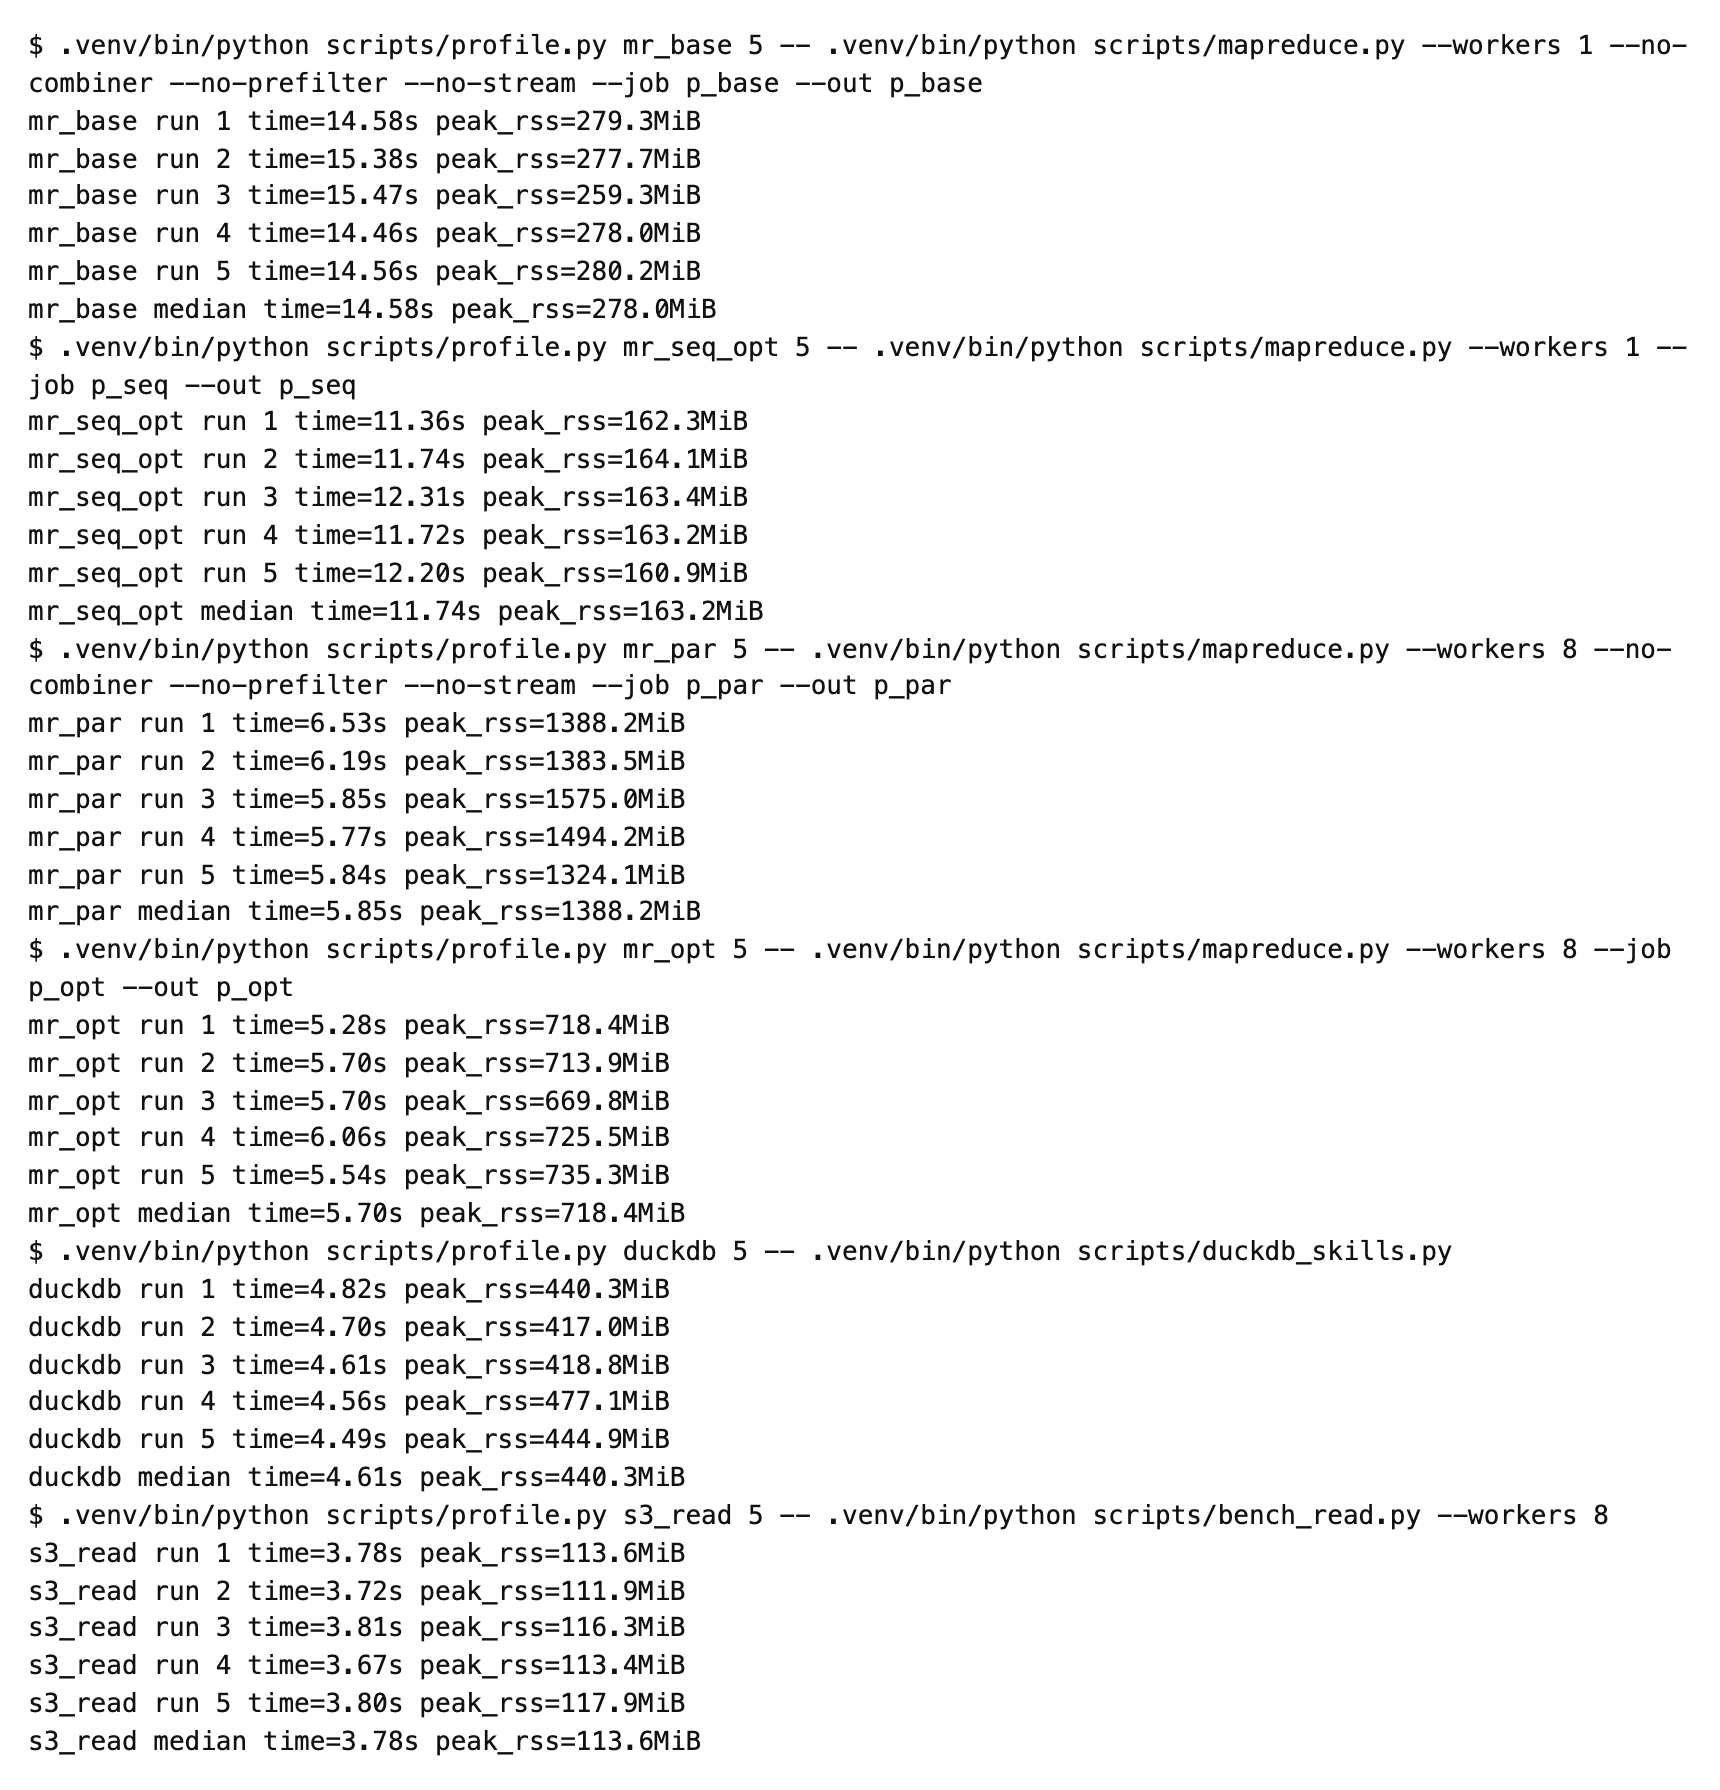
\includegraphics[width=\textwidth]{../screenshots/08_profile.png}
\caption{Выводы профилирования}
\end{figure}

Нижняя граница времени задается хранилищем. Одно чтение объекта без
обработки занимает 3,78 с, это около 224 МБ/с. RustFS работает в Docker на
одном SSD и собирает каждый блок из фрагментов EC 2+2. DuckDB тратит сверх
этого чтения 0,83 с, оптимизированный MapReduce 1,92 с. У MapReduce сверху
добавляются запуск процессов Python, фаза reduce и запись результатов.

DuckDB быстрее и экономнее по памяти, чем оптимизированный MapReduce. Он
разбирает CSV векторно на нескольких потоках внутри одного процесса. Свой
MapReduce запускает восемь процессов Python, и каждый занимает память под
интерпретатор, boto3 и свои буферы. Зато модель MapReduce переживает отказ
отдельной задачи, а задачи можно разнести по нескольким машинам. DuckDB
работает в одном процессе на одной машине.

Бонусная оптимизация дала такие результаты. Базовая версия обрабатывает
сплиты последовательно, держит сплит и копии всех его строк в памяти,
разбирает каждую строку CSV и выдает каждый ключ отдельно. Потоковое чтение
кусками по 1 МиБ, предфильтр по байтам роли и комбайнер в одном процессе
сократили время с 14,58 до 11,74 с, то есть на 19 процентов, а пик памяти с
278,0 до 163,2 МиБ, на 41 процент. Восемь процессов уменьшили время до
5,70 с, в 2,6 раза меньше базового. Память при этом выросла до 718,4 МиБ,
потому что одновременно работают восемь процессов. По сравнению с простым
распараллеливанием без других оптимизаций итоговая версия требует на 48
процентов меньше памяти, а время почти то же, 5,70 против 5,85 с. Эта
разница меньше разброса между запусками. Комбайнер сократил данные
шаффла со 191397 до 138585 записей, на 28 процентов.

\section{6. Влияние навыков на зарплату}

Для анализа берутся вакансии варианта с зарплатой в рублях, это 1255 из
1380 вакансий с зарплатой. Зарплата вакансии равна середине вилки или
единственной указанной границе. Если зарплата указана до вычета НДФЛ, она
умножается на 0,87, чтобы все суммы были на руки. Значения меньше 20000
рублей в месяц исключены как ошибки ввода, это 5 вакансий. Остается 1250 вакансий, у 995 из них
есть навыки. Медиана по этим 995 вакансиям 160000 рублей. Опыт до трех лет
требуют 56 процентов из них, дальше такие вакансии называются вакансиями
для начинающих.

Сначала вакансии сравниваются по уровню зарплаты и набору навыков. Они
делятся на четыре равные группы по зарплате.

\begin{table}[H]
\centering
\small
\setlength{\tabcolsep}{4pt}
\begin{tabular}{|c|L{1.7cm}|L{2.4cm}|L{1.6cm}|L{1.6cm}|L{1.9cm}|L{4.9cm}|}
\hline
Группа & Вакансий & Зарплата, рублей & Медиана & Навыков в среднем & Опыт до 3 лет, процентов & Частые навыки, вакансий \\
\hline
1 & 249 & 20000 и 100000 & 80000 & 6,2 & 92 & git 114, android 106, ios 99, flutter 62, kotlin 62 \\
\hline
2 & 249 & 100000 и 160000 & 130000 & 6,3 & 73 & android 128, git 104, ios 96, flutter 75, kotlin 71 \\
\hline
3 & 249 & 160000 и 250000 & 190000 & 6,1 & 47 & android 118, git 103, ios 98, kotlin 86, flutter 61 \\
\hline
4 & 248 & 250000 и 525000 & 291450 & 5,3 & 13 & kotlin 120, android 112, git 63, ios 62, android sdk 60 \\
\hline
\end{tabular}
\caption{Вакансии по четвертям зарплаты, в столбце зарплаты наименьшее и наибольшее значение}
\end{table}

В дорогих вакансиях меньше навыков, 5,3 против 6,2 в дешевых. Работодатель
опытного разработчика называет несколько главных технологий, а в вакансии
для начинающих перечисляет базовые инструменты. Git есть в 46 процентах
вакансий нижней группы и в 25 процентах верхней. Kotlin выходит на первое
место только в верхней группе, а Flutter пропадает из ее пяти частых навыков.

Прибавку от сочетания нужно считать от базы. Для пары база это более частый
навык пары, для тройки самая частая из трех вложенных пар. Частоты берутся
из результатов MapReduce в hh-lake. Прибавка равна медиане зарплаты
вакансий с сочетанием минус медиана вакансий с базой. Медиана по нескольким
вакансиям неустойчива, поэтому учитываются сочетания, которые есть минимум в
15 вакансиях с зарплатой. Таких 200 пар и 183 тройки.

\begin{code}
SELECT s1 || ' + ' || s2 AS combo, b.n, base, m1.med AS base_med, b.med,
       b.med - m1.med AS uplift
FROM (SELECT m2.*, CASE WHEN fa.freq > fb.freq OR (fa.freq = fb.freq AND s1 < s2)
                        THEN s1 ELSE s2 END AS base
      FROM m2 JOIN f1 fa ON fa.skill = s1 JOIN f1 fb ON fb.skill = s2
      WHERE m2.n >= 15) b
JOIN m1 ON m1.skill = base;
\end{code}

\begin{table}[H]
\centering
\small
\footnotesize
\setlength{\tabcolsep}{4pt}
\begin{tabular}{|L{5.4cm}|L{1.5cm}|L{4.4cm}|L{1.4cm}|L{2.0cm}|L{1.5cm}|}
\hline
Сочетание & С зарплатой & База и ее медиана & Медиана & Прибавка & Опыт до 3 лет \\
\hline
\multicolumn{6}{|l|}{Пары, повышающие медиану} \\
\hline
android + kotlin coroutines & 16 & android, 158300 & 250000 & 91700, 58 & 19 \\
coroutines + kotlin & 20 & kotlin, 187920 & 270000 & 82080, 44 & 20 \\
jetpack compose + kotlin & 21 & kotlin, 187920 & 252300 & 64380, 34 & 43 \\
dagger 2 + java & 18 & java, 156125 & 220000 & 63875, 41 & 33 \\
android + hilt & 16 & android, 158300 & 221850 & 63550, 40 & 13 \\
\hline
\multicolumn{6}{|l|}{Тройки, повышающие медиану} \\
\hline
dagger 2 + java + kotlin & 17 & java + kotlin, 160000 & 260000 & 100000, 63 & 29 \\
ios + solid + swift & 17 & ios + swift, 160000 & 250000 & 90000, 56 & 29 \\
android + mvi + mvvm & 15 & android + mvvm, 150000 & 217500 & 67500, 45 & 13 \\
android + kotlin + kotlin coroutines & 16 & android + kotlin, 187920 & 250000 & 62080, 33 & 19 \\
android + dagger 2 + java & 18 & android + java, 160000 & 220000 & 60000, 38 & 33 \\
\hline
\multicolumn{6}{|l|}{Пары, понижающие медиану} \\
\hline
android studio + kotlin & 21 & kotlin, 187920 & 95700 & $-$92220, $-$49 & 71 \\
flutter + kotlin & 18 & kotlin, 187920 & 110000 & $-$77920, $-$41 & 78 \\
kotlin + mvp & 24 & kotlin, 187920 & 110000 & $-$77920, $-$41 & 79 \\
ios + json api & 23 & ios, 150000 & 80000 & $-$70000, $-$47 & 70 \\
android studio + java & 17 & java, 156125 & 90000 & $-$66125, $-$42 & 76 \\
\hline
\multicolumn{6}{|l|}{Тройки, понижающие медиану} \\
\hline
android + android studio + kotlin & 15 & android + kotlin, 187920 & 90000 & $-$97920, $-$52 & 67 \\
android + kotlin + mvp & 17 & android + kotlin, 187920 & 110000 & $-$77920, $-$41 & 88 \\
android studio + java + kotlin & 16 & java + kotlin, 160000 & 87500 & $-$72500, $-$45 & 75 \\
android + android sdk + mvp & 15 & android + android sdk, 180000 & 110000 & $-$70000, $-$39 & 87 \\
android sdk + kotlin + mvp & 17 & android sdk + kotlin, 180000 & 110000 & $-$70000, $-$39 & 88 \\
\hline
\end{tabular}
\caption{Итоговая таблица. Медианы и прибавка в рублях на руки, прибавка также в процентах от базы, опыт до 3 лет в процентах вакансий сочетания}
\end{table}

Повышают зарплату навыки современного Android-стека. Это корутины Kotlin,
Jetpack Compose, внедрение зависимостей Dagger 2 и Hilt, архитектура MVI.
Пара android + kotlin coroutines поднимает медиану на 91700 рублей
относительно вакансий с Android. В iOS к тому же ведет SOLID, тройка ios +
solid + swift дает 250000 рублей против 160000 у ios + swift. В этих
сочетаниях вакансий для начинающих от 13 до 43 процентов при 56 процентах в
среднем по варианту.

Понижают зарплату Android Studio, MVP, JSON API и Flutter рядом с нативным
языком. Причина не в самих навыках. Это среда разработки, устаревшая
архитектура и базовые форматы, которые перечисляют в вакансиях для
начинающих, их там от 67 до 88 процентов. Сочетание flutter + kotlin
встречается в объявлениях младших кроссплатформенных разработчиков. Похожая
картина у троек git + objective-c + swift и git + ios + objective-c, они
понижают медиану на 61600 и 53950 рублей при 90 и 91 проценте вакансий для
начинающих. Таблица показывает связь навыков с зарплатой в объявлениях, а
не то, что изучение навыка само по себе меняет зарплату.

\section{7. Региональный анализ}

Выбраны Москва, Санкт-Петербург и Екатеринбург. После двух столиц в
Екатеринбурге больше всего вакансий варианта с зарплатой, 66. В Новосибирске
вакансий больше, 144 против 137, но с зарплатой только 46, а медиана по
малой выборке неустойчива.

\begin{table}[H]
\centering
\small
\begin{tabular}{|L{7.5cm}|c|c|c|}
\hline
Показатель & Москва & Санкт-Петербург & Екатеринбург \\
\hline
Вакансий варианта & 1752 & 592 & 137 \\
Доля от всех вакансий варианта, процентов & 46 & 16 & 4 \\
Вакансий с зарплатой & 522 & 179 & 66 \\
Нижний квартиль зарплаты, рублей & 140000 & 115000 & 102500 \\
Медиана зарплаты, рублей & 200000 & 160000 & 180000 \\
Верхний квартиль зарплаты, рублей & 277550 & 237450 & 300000 \\
Опыт до 3 лет, процентов & 32 & 42 & 58 \\
Удаленная работа, процентов & 42 & 34 & 32 \\
Вакансий с навыками & 1250 & 420 & 111 \\
Навыков в вакансии в среднем & 5,4 & 5,3 & 4,4 \\
\hline
\end{tabular}
\caption{Ключевые показатели регионов}\label{tab:reg1}
\end{table}

\begin{table}[H]
\centering
\small
\footnotesize
\setlength{\tabcolsep}{4pt}
\begin{tabular}{|l|L{5.1cm}|L{5.1cm}|L{5.1cm}|}
\hline
 & Москва & Санкт-Петербург & Екатеринбург \\
\hline
Навык 1 & kotlin 39, 243600 & android 43, 160000 & android 33, 250000 \\
Навык 2 & android 39, 200000 & kotlin 41, 186350 & git 32, 125000 \\
Навык 3 & ios 30, 180000 & ios 35, 160000 & ios 30, 250000 \\
Навык 4 & git 27, 177110 & swift 27, 190000 & kotlin 29, 250000 \\
Навык 5 & swift 26, 200000 & java 23, 160000 & swift 27, 275000 \\
\hline
Пара 1 & android + kotlin 27, 224460 & android + kotlin 31, 185000 & android + kotlin 23, 250000 \\
Пара 2 & ios + swift 20, 190000 & ios + swift 22, 195000 & ios + swift 19, 300000 \\
Пара 3 & android sdk + kotlin 17, 226200 & java + kotlin 21, 160000 & java + kotlin 18, 240000 \\
\hline
Тройка 1 & android + android sdk + kotlin 13, 225330 & android + java + kotlin 16, 160000 & android + java + kotlin 14, 300000 \\
Тройка 2 & android + java + kotlin 12, 230000 & android + android sdk + kotlin 12, 220000 & android + android sdk + kotlin 13, 300000 \\
Тройка 3 & android sdk + java + kotlin 9, 227230 & android sdk + java + kotlin 8, 150000 & android sdk + java + kotlin 13, 240000 \\
\hline
\end{tabular}
\caption{Частые навыки, пары и тройки. В ячейке доля вакансий региона с навыками в процентах и медиана зарплаты в рублях}\label{tab:reg2}
\end{table}

Таблицы построены одним SQL по тому же объекту S3. Ниже часть запроса для
пар внутри региона, навыки и тройки считаются так же.

\begin{code}
CREATE TABLE r AS SELECT seg.*, sal.salary FROM seg LEFT JOIN sal USING (vacancy_id)
WHERE seg.area IN ('Москва', 'Санкт-Петербург', 'Екатеринбург');
CREATE TABLE e AS SELECT vacancy_id, area, salary, unnest(skills) AS skill FROM r;
SELECT a.area, a.skill || ' + ' || b.skill AS combo, count(*) AS vacancies,
       count(a.salary) AS n_salary, median(a.salary) AS median_salary
FROM e a JOIN e b ON a.vacancy_id = b.vacancy_id AND a.skill < b.skill
GROUP BY ALL;
\end{code}

Москва дает почти половину вакансий варианта и самую высокую медиану,
200000 рублей. Вакансий для начинающих там меньше всего, 32 процента, а
удаленной работы больше всего, 42 процента. Kotlin в Москве первый навык, и
вакансии с ним дают медиану 243600 рублей. Столичный рынок ищет опытных
Android-разработчиков на современном стеке.

В Санкт-Петербурге медиана на 20 процентов ниже московской, 160000 рублей.
Вакансий для начинающих больше, 42 процента, а связка Android и Kotlin
встречается чаще, чем в Москве, в 31 проценте вакансий. Петербургский рынок
сильнее смещен к Android и к Java рядом с Kotlin.

Екатеринбург самый неоднородный. Вакансий для начинающих 58 процентов,
навыков в вакансии меньше всего, 4,4, а разброс зарплат самый широкий, от
102500 до 300000 рублей между квартилями. Медиана 180000 рублей выше
петербургской за счет вакансий с опытом от 3 до 6 лет, их медиана 300000
рублей. С опытом от 1 до 3 лет там предлагают 155000 рублей, в столицах
150000.
В Екатеринбурге чаще, чем в столицах, встречаются Flutter, 19 процентов
вакансий, Dart, 16 процентов, ООП, 17 процентов, и git, 32 процента. Это
признаки кроссплатформенных проектов и вакансий для начинающих. Медианы
по навыкам Екатеринбурга основаны на 3 и 18 вакансиях с зарплатой и
показывают только направление.

Исходный код всех программ, логи, результаты и этот отчет опубликованы в
репозитории \url{https://github.com/Gegerout/data-engineering-lab3}.
Команды запуска описаны в README репозитория.


\end{document}
